\section{Analytical Solutions}
	\subsection{Rectangular quantum well}
		\begin{figure}[!h]
			\centering
			\begin{tikzpicture}[scale=4,cap=round,>=latex]
	\draw [<->] (-2, 1.5) -- (-2, 0) -- (1.5, 0);
	\node [left] at (-2, 1.5) {$U$};
	\node [below] at (1.5, 0) {$z$};
	
	\draw [line width=1.5] (-2, 1) -- (-1, 1) -- (-1, 0) -- (0, 0) -- (0, 1) -- (1, 1);
	\draw [dashed] (-1, 1) -- (-1, 1.5);
	\draw [dashed] (0, 1) -- (0, 1.5);
	
	\node [left] at (-2, 1) {$U_0$};
	\node [below] at (-1, 0) {$-\frac{d}{2}$};
	\node [below] at (0, 0) {$\frac{d}{2}$};
	
	\node at (-1.5, 1.2) {I};
	\node at (-0.5, 1.2) {II};
	\node at (0.5, 1.2) {III};										
\end{tikzpicture}
			\caption{Finite rectangular quantum well}
		\end{figure}
		
		\begin{equation}
			\hat{H} = \frac{\hbar}{2m} \frac{\partial^2}{\partial z^2} + U(z)
		\end{equation}
		
		\begin{align}
			\text{II:}&\qquad E\Psi = \frac{\hbar}{2m} \frac{\partial^2}{\partial z^2}\Psi \\
			\text{I \& III:}& \qquad E\Psi = \frac{\hbar}{2m} \frac{\partial^2}{\partial z^2}\Psi + U_0\Psi 
		\end{align}
				
		Solutions for each area:
		\begin{align}
			\text{I:}&\qquad \Psi = A e^{+ik'z} + B e^{-ik'z} \\
			\text{II:}&\qquad \Psi = C e^{+ikz} + D e^{-ikz} \\
			\text{III:}&\qquad \Psi = F e^{+ik'z} + G e^{-ik'z} \\
			&\qquad k = \sqrt{\frac{2mE}{\hbar^2}};\qquad k' = \sqrt{\frac{2m(E-U_0)}{\hbar^2}}
		\end{align}
		\subsubsection{Bound states}
			For $E < U_0$, $k'$ is imaginary, meaning that
			\begin{align}
				\lim_{z \to -\infty} Ae^{+ik'z} = \lim_{z \to -\infty} Ae^{-sz} = \infty \\
				\lim_{z \to \infty} Ge^{-ik'z} = \lim_{z \to \infty} Ae^{sz} = \infty
			\end{align}
			Which is not physical, meaning that 
			\begin{equation}
				A = G = 0
			\end{equation}
			We have bounadary conditions at $z = -\frac{d}{2}$ and $z = \frac{d}{2}$:
			\begin{align}
				\Psi_I = \Psi_{II}|_{z=-\frac{d}{2}};&\qquad  \Psi_I' = \Psi_{II}'|_{z=-\frac{d}{2}} \\
				\Psi_{II} = \Psi_{III}|_{z=\frac{d}{2}};&\qquad  \Psi_{II}' = \Psi_{III}'|_{z=\frac{d}{2}}
			\end{align}
			Which can be written as:
			\begin{align}
				\kappa = ik' =& \sqrt{\frac{2m(U_0-E)}{\hbar^2}} \\
				Be^{-\kappa\frac{d}{2}} = Ce^{-ik\frac{d}{2}} + De^{+ik\frac{d}{2}}&\\
				-B\kappa e^{-\kappa\frac{d}{2}} &= ikCe^{-ik\frac{d}{2}} - ikde^{+ik\frac{d}{2}}\\
				Fe^{-\kappa\frac{d}{2}} = Ce^{+ik\frac{d}{2}} + De^{-ik\frac{d}{2}}&\\
				-F\kappa e^{-\kappa\frac{d}{2}} &= ikCe^{+ik\frac{d}{2}} - ikde^{-ik\frac{d}{2}}\\
			\end{align}
			Or in matrix form:
			\begin{equation}
				\begin{pmatrix}
				e^{-\kappa\frac{d}{2}}			&	-e^{-ik\frac{d}{2}}	&	-e^{ik\frac{d}{2}}	&	0 \\ 
				0	&	-e^{-ik\frac{d}{2}}	&	-e^{-ik\frac{d}{2}}	&	e^{-\kappa \frac{d}{2}} \\
				-\kappa e^{-\kappa \frac{d}{2}}	& -ike^{-ik\frac{d}{2}}	& +ike^{ik\frac{d}{2}}	& 0 \\
				0	& +ike^{ik\frac{d}{2}}	& -ike^{ik\frac{d}{2}}	& 	-\kappa e^{-\kappa\frac{d}{2}}	& \\
				\end{pmatrix}
				\begin{pmatrix}
				B \\
				C \\
				D \\
				F \\
				\end{pmatrix}
				=
				\begin{pmatrix}
				0 \\
				0 \\
				0 \\
				0 \\
				\end{pmatrix}			
			\end{equation}
			\hl{Direct solution?}
			Since our system is symmetric, we can simplify the system of equations:
			
			\begin{align}
				|\Psi|^2_{-\frac{d}{2}} =& |\Psi|^2_{\frac{d}{2}} \Rightarrow\\
				\Psi(z) = \Psi(-z) \qquad\text{or}&\qquad \Psi(z) = -\Psi(-z)
			\end{align}
			Which means that our system can have either symmetric or antisymmetric solutions:
			\begin{align}
				\Psi_{II}& = C e^{ikz} + D e^{-ikz} = C' \cos(kz) + D' \sin(kz) \\
				\Psi_{I}& = B e^{-\kappa z} \\
				\Psi_{III}& = F e^{\kappa z} \\		
			\end{align}
			Where $C'\cos(kz)$ and $A=F$ correspond to symmetric solutions and $D' \sin(kz)$ and $A = -F$~--- to antisymmetric solutions.
			
			\paragraph{Symmetric solutions}
				
				\begin{align}
					Be^{-\kappa \frac{d}{2}} &= C' \cos(\frac{kd}{2}) \\
					\kappa Be^{-\kappa \frac{d}{2}} &= kC' \sin(\frac{kd}{2})			
				\end{align}
				Or in matrix form:
				\begin{equation}
				\begin{pmatrix}
				e^{-\kappa \frac{d}{2}}			&	-\cos{\frac{kd}{2}}	\\ 
				\kappa e^{-\kappa \frac{d}{2}}	&	-k\sin{\frac{kd}{2}}	\\
				\end{pmatrix}
				\begin{pmatrix}
				B \\
				C' \\
				\end{pmatrix}
				=
				\begin{pmatrix}
				0 \\
				0 \\
				\end{pmatrix}			
				\end{equation}
				This system has non-trivial solutions when the determinant of the matrix is equal to zero:
				\begin{align}
					\begin{vmatrix}
						e^{-\kappa \frac{d}{2}}			&	-\cos{\frac{kd}{2}}	\\ 
						\kappa e^{-\kappa \frac{d}{2}}	&	-k\sin{\frac{kd}{2}}	\\
					\end{vmatrix}
					=& -e^{-\kappa\frac{d}{2}} k\sin{\frac{kd}{2}} + \kappa e^{-\kappa \frac{d}{2}} \cos{\frac{kd}{2}} =\\
					=& -k\sin(\frac{kd}{2}) + \kappa\cos(\frac{kd}{2}) = 0 \\
					\frac{k}{\kappa} =& \cot(\frac{kd}{2}) \label{symtranceq}
				\end{align}
				
				With solutions to \ref{symtranceq} defining the number of bound states in the quantum well. 
				\begin{figure}[!h]
					\centering
					
\begin{tikzpicture}[scale=2,cap=round,>=latex]
	\draw [line width=2] (-2, -2) -- (-2, 2) -- (2, 2) -- (2, -2) -- (-2, -2);
	
	\node at (0, 0) {placeholder};
\end{tikzpicture}
					\caption{Graphical solution to \ref{symtranceq}}
				\end{figure}
				
				In the limit case of $U_0 \rightarrow \infty$,
				\begin{align}
					\frac{k}{\kappa} =& \cot(\frac{kd}{2}),\qquad \kappa \rightarrow \infty \Rightarrow \\
					\cot(\frac{kd}{2}) =& 0 \Rightarrow\qquad	\cos(\frac{kd}{2}) = 0 \Rightarrow\\
					\frac{kd}{2} =& \frac{\pi}{2} + \pi n \\
					k_n =& \frac{\Pi + 2\pi n}{d} \\
					E_n =& \frac{\hbar^2}{2m}\frac{1}{d^2}\left(\pi + 2\pi n\right)^2
				\end{align}
				Which corresponds to the symmetric solutions found earlier to the infinite quantum well problem.
				
			\paragraph{Antisymmetric solutions}
				
				\begin{align}
					Be^{-\kappa \frac{d}{2}} &= D' \sin(\frac{kd}{2}) \\
					\kappa Be^{-\kappa \frac{d}{2}} &= -kD' \cos(\frac{kd}{2})			
				\end{align}
				Or in matrix form:
				\begin{equation}
				\begin{pmatrix}
				e^{-\kappa \frac{d}{2}}			&	-\sin{\frac{kd}{2}}	\\ 
				\kappa e^{-\kappa \frac{d}{2}}	&	k\cos{\frac{kd}{2}}	\\
				\end{pmatrix}
				\begin{pmatrix}
				B \\
				D' \\
				\end{pmatrix}
				=
				\begin{pmatrix}
				0 \\
				0 \\
				\end{pmatrix}			
				\end{equation}
				This system has non-trivial solutions when the determinant of the matrix is equal to zero:
				\begin{align}
					\begin{vmatrix}
						e^{-\kappa \frac{d}{2}}			&	-\sin{\frac{kd}{2}}	\\ 
						\kappa e^{-\kappa \frac{d}{2}}	&	k\cos{\frac{kd}{2}}	\\
					\end{vmatrix}
					=& e^{-\kappa\frac{d}{2}} k\cos{\frac{kd}{2}} + \kappa e^{-\kappa \frac{d}{2}} \sin{\frac{kd}{2}} =\\
					=& k\cos(\frac{kd}{2}) + \kappa\sin(\frac{kd}{2}) = 0 \\
					\frac{k}{\kappa} =& -\tan(\frac{kd}{2}) \label{antisymtranceq}
				\end{align}
				
				With solutions to \ref{antisymtranceq} defining the number of bound states in the quantum well. 
				\begin{figure}[!h]
					\centering
					
\begin{tikzpicture}[scale=2,cap=round,>=latex]
	\draw [line width=2] (-2, -2) -- (-2, 2) -- (2, 2) -- (2, -2) -- (-2, -2);
	
	\node at (0, 0) {placeholder};
\end{tikzpicture}
					\caption{Graphical solution to \ref{antisymtranceq}}
				\end{figure}
				
				In the limit case of $U_0 \rightarrow \infty$,
				\begin{align}
					\frac{k}{\kappa} =& -\tan(\frac{kd}{2}),\qquad \kappa \rightarrow \infty \Rightarrow \\
					\tan(\frac{kd}{2}) =& 0 \Rightarrow\qquad	\sin(\frac{kd}{2}) = 0 \Rightarrow\\
					\frac{kd}{2} =& \pi n \\
					k_n =& \frac{2\pi n}{d} \\
					E_n =& \frac{\hbar^2}{2m}\frac{1}{d^2}\left(2\pi n\right)^2
				\end{align}
				Which corresponds to antisymmetric solutions found earlier to the infinite quantum well problem.		
				
			\begin{figure}[!h]
				\centering
				
\begin{tikzpicture}[scale=2,cap=round,>=latex]
	\draw [line width=2] (-2, -2) -- (-2, 2) -- (2, 2) -- (2, -2) -- (-2, -2);
	
	\node at (0, 0) {placeholder};
\end{tikzpicture}
				\caption{Quantum well bound state wave functions}
			\end{figure}
			For $E > U_0$, the states of the system form a continuous spectrum of waves propagating in either direction.
		\subsubsection{Propagating states in a system of potential barriers}
			\begin{figure}[!h]
				\centering
				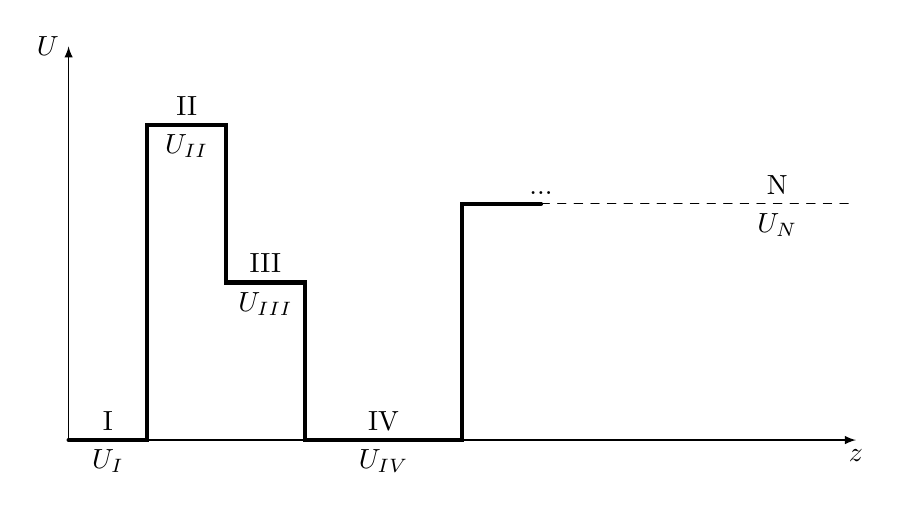
\begin{tikzpicture}[scale=1,cap=round,>=latex]
	\draw [<->] (-5, 5) -- (-5, 0) -- (5, 0);
	\node [left] at (-5, 5) {$U$};
	\node [below] at (5, 0) {$z$};
	
	\draw [line width=1.5] (-5, 0) -- (-4, 0) -- 
							(-4, 4) -- (-3, 4) -- 
							(-3, 2) -- (-2, 2) --
							(-2, 0) -- (0, 0) --
							(0, 3) -- (1, 3);
	\draw [dashed] (1, 3) -- (5, 3);
	
	\node [above] at (-4.5, 0) {I};
	\node [below] at (-4.5, 0) {$U_I$};

	\node [above] at (-3.5, 4) {II};
	\node [below] at (-3.5, 4) {$U_{II}$};
	
	\node [above] at (-2.5, 2) {III};
	\node [below] at (-2.5, 2) {$U_{III}$};

	\node [above] at (-1, 0) {IV};
	\node [below] at (-1, 0) {$U_{IV}$};
	
	\node [above] at (1, 3) {...};
		
	\node [above] at (4, 3) {N};
	\node [below] at (4, 3) {$U_{N}$};


	%\node [below] at (-1, 0) {$-\frac{d}{2}$};
	%\node [below] at (0, 0) {$\frac{d}{2}$};
	
\end{tikzpicture}
				\caption{System of potential barriers}
			\end{figure}			
			The system and be separated into two cases: propagation through a region, and reflection/transmission through a barrier, these cases correspond to solutions of the Shr\"odinger equation in each of the regions and to the boundary conditions between the regions.
			
			The wavefunction at each point of the system can be written as a sum of forward and backward propagating waves:
			\begin{align}
				\Psi|_{z=z_{0}} =& Ae^{ikz_0} + Be^{-ikz_0} \\
				\Psi|_{z=z_{0}+d} =& Ae^{ikz_0}e^{ikd} + Be^{-ikz_0}e^{-ikd}				
			\end{align}
			or, in vector form:
			\begin{equation}
				\Psi = 
				\begin{pmatrix}
				A_+ \\
				A_- \\
				\end{pmatrix}
			\end{equation}
			
			In that case, equations \hl{REF} can be rewritten as a matrix equation:
			\begin{align}
				\Psi|_{z=z_{0}} =& 
				\begin{pmatrix}
					A_+ \\
					A_- \\
				\end{pmatrix} \\
				\Psi|_{z=z_{0}+d} =&
				\begin{pmatrix}
					A_+' \\
					A_-' \\
				\end{pmatrix}				
				= \begin{pmatrix}
					A_+ \\
					A_- \\
				\end{pmatrix} \hat{M} = \Psi|_{z=z_{0}} \hat{M}
			\end{align}
			
			If both $z_0$ and $z_0 + d$ correspond to the same region of the system of barriers, then matrix $\hat{M}$ is simply a propagation matrix:
			\begin{equation}
				\hat{P} = \begin{pmatrix}
				e^{ikd} & 0 \\
				0		& e^{-ikd}
				\end{pmatrix}
			\end{equation}
			
			To build a matrix corresponding to the boundary between regions, he have to start with a different basis, in which we can easily write the boundary conditions:
			
			\begin{align}
				\begin{pmatrix}	
					\Psi_{I} \\
					\frac{\partial \Psi_{I}}{\partial z}
				\end{pmatrix} =& 
				\hat{I} \begin{pmatrix}	
					\Psi_{II} \\
					\frac{\partial \Psi_{II}}{\partial z}
				\end{pmatrix} \\
				\hat{I} =& \begin{pmatrix}
					\hl{explicit} & \hl{explicit} \\
					\hl{explicit} & \hl{explicit} 					
					\end{pmatrix}
			\end{align}
			
			The basis	$\left(\begin{smallmatrix}	
				\Psi_{I} \\
				\frac{\partial \Psi_{I}}{\partial z}
			\end{smallmatrix}\right)$ can be easily written in terms of the basis $\left(\begin{smallmatrix}
				A_+' \\
				A_-' \\
			\end{smallmatrix}\right)$:
			
			\begin{align}
				\Psi =& A_+ e^{ikz} + A_- e^{-ikz} \\
				\frac{\partial \Psi}{\partial z} =& ikA_+ e^{ikz} - ikA_- e^{-ikz} \\
				\begin{pmatrix}	
					\Psi \\
					\frac{\partial \Psi}{\partial z}
				\end{pmatrix} =& 
				\begin{pmatrix}
					1 & 1 \\
					ik & -ik \\
				\end{pmatrix}
				\begin{pmatrix}
					A_+ \\
					A_- \\
				\end{pmatrix} = \hat{S} 
				\begin{pmatrix}
					A_+ \\
					A_- \\
				\end{pmatrix}
			\end{align}
			
			Meaning that 
			\begin{align}
				\begin{pmatrix}	
					\Psi \\
					\frac{\partial \Psi}{\partial z}
				\end{pmatrix}
				= \hat{S} 
				\begin{pmatrix}
					A_+ \\
					A_- \\
				\end{pmatrix} \qquad\&&\qquad
				\begin{pmatrix}
					A_+ \\
					A_- \\
				\end{pmatrix} = \hat{S}^-1
				\begin{pmatrix}	
					\Psi \\
					\frac{\partial \Psi}{\partial z}
				\end{pmatrix} \\
				\begin{pmatrix}	
					\Psi_{I} \\
					\frac{\partial \Psi_{I}}{\partial z}
				\end{pmatrix} =& 
				\hat{I} \begin{pmatrix}	
					\Psi_{II} \\
					\frac{\partial \Psi_{II}}{\partial z}
					\end{pmatrix} \\
				\hat{S} 
				\begin{pmatrix}
					A_{I+} \\
					A_{I-} \\
				\end{pmatrix} =& 
				\hat{I}\hat{S} 
				\begin{pmatrix}
					A_{II+} \\
					A_{II-} \\
				\end{pmatrix} \\
				\begin{pmatrix}
					A_{I+} \\
					A_{I-} \\
				\end{pmatrix} =& 
				\hat{S}^{-1}\hat{I}\hat{S} 
				\begin{pmatrix}
					A_{II+} \\
					A_{II-} \\
				\end{pmatrix} \\
				\begin{pmatrix}
					A_{I+} \\
					A_{I-} \\
				\end{pmatrix} =& 
				\hat{M} 
				\begin{pmatrix}
					A_{II+} \\
					A_{II-} \\
				\end{pmatrix},\qquad \hat{M} = \hat{S}^{-1}\hat{I}\hat{S} \\
				\hl{\det{\hat{M}}} =& 1
			\end{align}
			Meaning that we can represent a whole series of potential wells and barriers as a product of their \textit{transfer} matricies:
			\begin{equation}
				\Psi_n = \hat{T_n}\hat{T_{n-1}}...\hat{T_2}\hat{T_1}\Psi_0, \qquad \hat{T_i} = \hat{M}_{i-1\rightarrow i}\hat{P_i} 
			\end{equation}
			
			Transfer matricies can also be used to find the bound states or eigenmodes of the system:
			\hl{Wait, what?}
			\begin{align}
				\hat{\Psi}_{\frac{d}{2}} =& \hat{\Psi}_{-\frac{d}{2}} \\
				\begin{pmatrix}
					Ae^{-\kappa \frac{d}{2}} \\
					-\kappa Ae^{-\kappa \frac{d}{2}} \\
				\end{pmatrix} =& \hat{T} 
				\begin{pmatrix}
					Be^{-\kappa \frac{d}{2}} \\
					\kappa Ae^{-\kappa \frac{d}{2}} \\
				\end{pmatrix}
			\end{align}
			
			Using transfer matricies, the calculation of an electron's probability of tunneling through a barrier is equivalent to solving the following matrix equation:
			\begin{align}
				\begin{pmatrix}
					t \\
					0
				\end{pmatrix} = \hat{M}
				\begin{pmatrix}
					1 \\
					r
				\end{pmatrix} \\
				r  = -\frac{M_{21}}{M_{22}} \\
				t = \frac{1}{M_{22}}
			\end{align}
	\subsection{Harmonic oscillator}
	\subsection{Spherically symmetric potential}
	\newpage
	\subsection{Problems}
		\subsubsection{Rectangular quantum well}
			\paragraph{Double quantum well}
				\begin{figure}[!h]
					\centering
					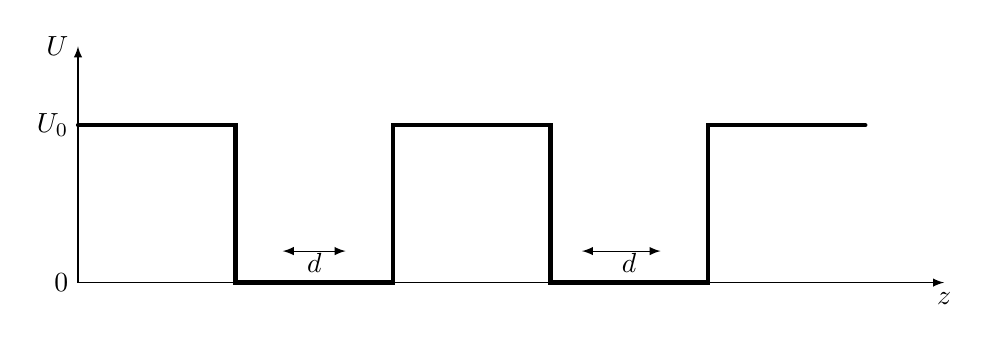
\begin{tikzpicture}[scale=2,cap=round,>=latex]
	\draw [<->] (-2, 1.5) -- (-2, 0) -- (3.5, 0);
	\node [left] at (-2, 1.5) {$U$};
	\node [below] at (3.5, 0) {$z$};
	
	\draw [line width=1.5] (-2, 1) -- (-1, 1) -- 
							(-1, 0) -- (0, 0) -- 
							(0, 1) -- (1, 1) --
							(1, 0) -- (2, 0) --
							(2, 1) -- (3, 1);
							
	\node [left] at (-2, 1) {$U_0$};
	\node [left] at (-2, 0) {$0$};	
	
	\node [above] at (-0.5, 0) {$d$};
	\draw [<->] (-0.7, 0.2) -- (-0.3, 0.2);
		
	\node [above] at (1.5, 0) {$d$};	
	\draw [<->] (1.2, 0.2) -- (1.7, 0.2);
										
\end{tikzpicture}
					\caption{Double quantum well}
				\end{figure}
				
				Calculate the eigenstates.
			\paragraph{Double quantum barrier}
				\begin{figure}[!h]
					\centering
					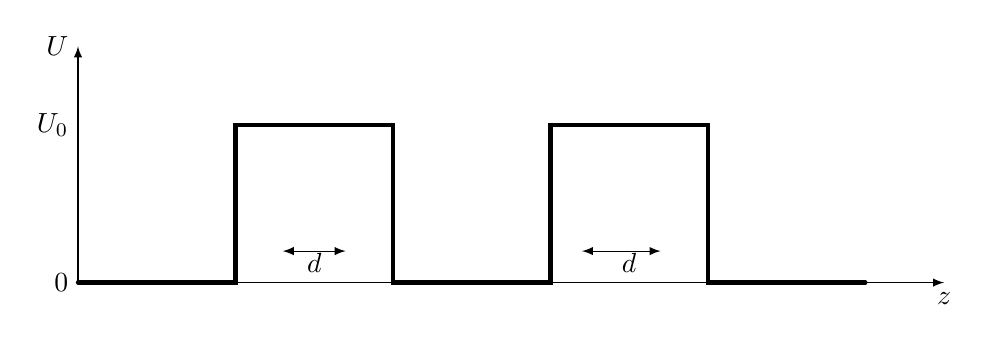
\begin{tikzpicture}[scale=2,cap=round,>=latex]
	\draw [<->] (-2, 1.5) -- (-2, 0) -- (3.5, 0);
	\node [left] at (-2, 1.5) {$U$};
	\node [below] at (3.5, 0) {$z$};
	
	\draw [line width=1.5] (-2, 0) -- (-1, 0) -- 
							(-1, 1) -- (0, 1) -- 
							(0, 0) -- (1, 0) --
							(1, 1) -- (2, 1) --
							(2, 0) -- (3, 0);
							
	\node [left] at (-2, 1) {$U_0$};
	\node [left] at (-2, 0) {$0$};	
	
	\node [above] at (-0.5, 0) {$d$};
	\draw [<->] (-0.7, 0.2) -- (-0.3, 0.2);
		
	\node [above] at (1.5, 0) {$d$};	
	\draw [<->] (1.2, 0.2) -- (1.7, 0.2);
										
\end{tikzpicture}
					\caption{Double quantum barrier system}
				\end{figure}
				
				Calculate the probability of a an electron tunneling through a system of two potential barriers.			
			\paragraph{Minimal transistor size}
				\begin{figure}[!h]
					\centering
					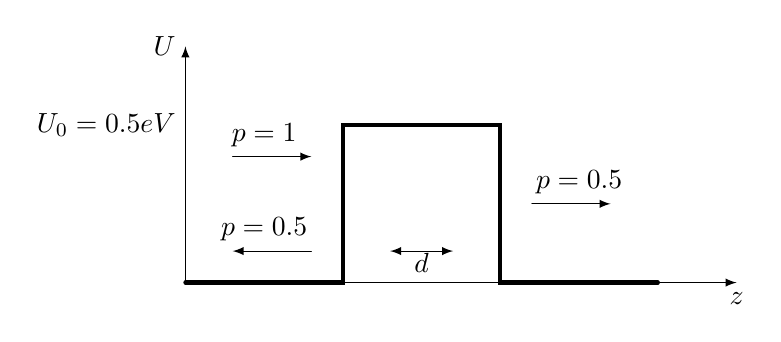
\begin{tikzpicture}[scale=2,cap=round,>=latex]
	\draw [<->] (-2, 1.5) -- (-2, 0) -- (1.5, 0);
	\node [left] at (-2, 1.5) {$U$};
	\node [below] at (1.5, 0) {$z$};
	
	\draw [line width=1.5] (-2, 0) -- (-1, 0) -- (-1, 1) -- (0, 1) -- (0, 0) -- (1, 0);
	
	\node [above] at (-0.5, 0) {$d$};
	\draw [<->] (-0.7, 0.2) -- (-0.3, 0.2);	
	
	\node [left] at (-2, 1) {$U_0 = 0.5\si{eV}$};

	\draw [->] (-1.7, 0.8) -- (-1.2, 0.8);
	\node [above] at (-1.5, 0.8) {$p = 1$};
		
	\draw [<-] (-1.7, 0.2) -- (-1.2, 0.2);
	\node [above] at (-1.5, 0.2) {$p = 0.5$};

	\draw [->] (0.2, 0.5) -- (0.7, 0.5);	
	\node [above] at (0.5, 0.5) {$p = 0.5$};
												
\end{tikzpicture}
					\caption{Model transistor}
				\end{figure}
							
				Calculate the size of a quantum barrier at which an electron's probability of tunneling through is equal to $0.5$.
				\begin{align}
					m_{el} \approx& 0.3 m_0 \\
					m_0 \approx& 10^{-30}\si{kg} \\
					p =& |\Psi|^2
				\end{align}
			